\documentclass[11pt]{article}

\usepackage[a4paper,margin=2.3cm]{geometry}
\usepackage{graphicx}
\usepackage{booktabs}
\usepackage{amsmath}
\usepackage{hyperref}
\usepackage{xcolor}
\usepackage{caption}
\usepackage{titlesec}
\usepackage{authblk}
\usepackage{setspace}
\usepackage[numbers,sort&compress]{natbib}

\hypersetup{colorlinks=true, linkcolor=blue!45!black, urlcolor=blue!45!black, citecolor=blue!45!black}
\captionsetup{font=small, labelfont=bf}
\titleformat{\section}{\normalfont\large\bfseries}{\thesection.}{0.5em}{}
\titleformat{\subsection}{\normalfont\bfseries}{\thesubsection.}{0.5em}{}
\onehalfspacing

\title{\textbf{Probabilistic dengue and chikungunya forecasting in Brazil:\\
metric-dependent model rankings, regime-shift fragility, and conformal ensembles}}
\author[1]{Author One}
\author[1]{Author Two}
\affil[1]{Institution (\texttt{DRAFT: placeholder authors and affiliations})}
\date{\today}

\begin{document}
\maketitle

\begin{abstract}
\noindent
Dengue is expanding across Brazil, and 2024 produced a record epidemic of roughly four times any
prior year. Accurate, well-calibrated probabilistic forecasts support preparedness, but the
relative merits of statistical, machine-learning, deep-learning, and mechanistic approaches for
this task are unsettled, especially under the distribution shift an outbreak year imposes. We
report a reproducible, leakage-controlled comparison of five probabilistic forecasting model
families for the 3rd Infodengue--Mosqlimate Dengue Challenge (IMDC 2026), which requires weekly,
state-level forecasts with full predictive intervals for the 26 mandatory Brazilian states. All
models are evaluated through a single backtesting harness over four official retrospective seasons,
one of which contains the 2024 outbreak, and scored by the weighted interval score (WIS). We report
four results with implications beyond this challenge. First, no model is best across seasons: a
global recurrent network is the most accurate model in normal seasons yet the worst on the 2024
outlier, whereas an ensemble never incurs any member's worst-season failure. Second, the identity
of the best model depends on the evaluation metric, because magnitude-weighted mean WIS and
scale-free normalized WIS reward accuracy on different subsets of a highly skewed set of states.
Third, a conformal recalibration of the ensemble intervals improves accuracy and calibration at
negligible cost (mean WIS 1281 to 1216, normalized WIS 0.585 to 0.555, out-of-sample reduction of
5.5 percent), acting as asymmetric insurance against catastrophic under-prediction. Fourth, added
model complexity did not pay: observed-climate covariates and hierarchical spatial pooling both
failed to improve forecasts, and an internal-holdout hyperparameter gain reversed on the true
backtest. The best model is disease-specific: for chikungunya, gradient boosting alone outperforms
the ensemble. All code, the backtesting harness, per-state scored predictions, and validated
submissions for four official tracks are released, with an automated test suite covering leakage,
scoring, and every model.
\end{abstract}

\section*{Author summary}
\noindent
Brazil carries one of the world's largest dengue burdens, and 2024 brought an epidemic without
precedent in the national record. Public-health agencies increasingly rely on forecasts that state
not just a single predicted number of cases but a full range of plausible outcomes with calibrated
uncertainty. Which forecasting method to trust is an open question, particularly during an
exceptional season when accurate forecasts matter most. We compared five families of models,
ranging from simple seasonal baselines to gradient boosting, deep learning, and a mechanistic
epidemic model, on identical retrospective tests across four dengue seasons in all 26 mandatory
Brazilian states. We found that no method is best everywhere: the deep-learning model was the most
accurate in ordinary seasons but failed badly during the 2024 outbreak, while a simple ensemble
that averages the models was the most dependable. We also found that the apparent winner changes
depending on how performance is scored, a caution for forecasting leaderboards. Finally, a light
statistical recalibration of the ensemble's uncertainty improved both accuracy and reliability, and
adding more data or model complexity did not help. Our full pipeline is openly available.

\section{Introduction}
Dengue is among the fastest-spreading mosquito-borne diseases, and Brazil bears one of the largest
national burdens \citep{lowe2021,colon2021}. The 2024 season broke the national record by a wide
margin, with a peak of 440{,}538 reported cases in a single epidemiological week and an annual total
near 6.67 million, roughly four times the next-largest year on record. Transmission is shaped by
climate, and the 2023--24 El Ni\~no is one of several drivers implicated in the surge. Against this
background, arboviral forecasting has moved from point prediction toward full probabilistic
forecasts, motivated by the recognition that preparedness decisions depend on the entire predictive
distribution rather than a single expected value \citep{johansson2019,cramer2022}.

The Infodengue--Mosqlimate Dengue Challenge (IMDC) operationalizes this shift. It invites teams to
submit weekly, state-level probabilistic forecasts with prescribed quantiles, scored by the weighted
interval score, following the precedent of the inaugural 2024 edition \citep{araujo2026}. The
challenge exposes a question that the wider forecasting literature has not resolved for this
setting: given statistical, machine-learning (ML), deep-learning (DL), and mechanistic approaches,
which forecast best, and how robustly, when a season can depart by an order of magnitude from
anything in the training record?

We address this with a controlled comparison built for reproducibility and for honest evaluation
under distribution shift. Every model is fit and scored through one backtesting harness that
enforces leakage safety and applies the same scoring code to all forecasts, over the four official
retrospective seasons (2022--23 through 2025--26) for the 26 mandatory states. We make the following
contributions.

\begin{enumerate}
\item We show that model rankings are season-dependent and, in the outbreak year, invert: the model
that is best on average can be the least reliable exactly when reliability matters most
(Section~\ref{sec:noseason}).
\item We show that the identity of the best model depends on whether skill is weighted by case
magnitude or by forecasting unit, a consequence of real cross-state heterogeneity rather than an
artifact, and we argue for reporting both (Section~\ref{sec:metric}).
\item We introduce a conformal recalibration of the ensemble intervals that improves accuracy and
calibration at negligible cost and functions as asymmetric insurance against catastrophic
under-prediction (Section~\ref{sec:conformal}).
\item We document informative negative results: added covariates, hierarchical pooling, and
hyperparameter tuning each failed to improve forecasts, which clarifies where the predictable signal
in this problem lies (Section~\ref{sec:negative}).
\item We show that the best model is disease-specific, using chikungunya as a contrasting target
(Section~\ref{sec:chik}), and we release the complete, tested pipeline.
\end{enumerate}

\section{Results}

\subsection{Study design and data}\label{sec:design}
We forecast weekly dengue case counts per state across the 2022--23 through 2025--26 seasons for the
26 mandatory Brazilian states (Espírito Santo is excluded per the challenge specification). Each of
the four backtest seasons is defined by an official training cutoff and a target window; a confirmed
15-week gap separates each training cutoff from the start of its evaluation window, reflecting the
reporting delay a real forecaster faces (Fig~\ref{fig:overview}). Forecasts are submitted as nine
quantiles per state and week, from which the four central prediction intervals (50, 80, 90, and 95
percent) are formed. All covariate access, feature construction, and model fitting are filtered to
data at or before each training cutoff, and this discipline is enforced by automated tests rather
than by convention (Section~\ref{sec:methods}). The four seasons differ by an order of magnitude in
difficulty. The 2023--24 season (fold 2), which contains the 2024 outbreak, is the hardest for every
model, and the 2025--26 season (fold 4) is only partially resolved in the available data and is
reported separately.

\begin{figure}[t]
\centering
\includegraphics[width=0.92\textwidth]{../results/figures/national_weekly_trends.png}
\caption{\textbf{National weekly dengue trend and study design.} Weekly reported dengue cases
aggregated to the national level, 2010--2026. The 2024 season stands roughly four times above any
prior year. Model evaluation uses four official retrospective seasons, each with a training cutoff,
a 15-week reporting gap, and a target window; forecasts are scored only on the target window.
Figure to be extended with an explicit fold-timeline panel and a state map.}
\label{fig:overview}
\end{figure}

\subsection{No single model dominates across seasons}\label{sec:noseason}
Table~\ref{tab:byfold} reports mean WIS by model and season, and Fig~\ref{fig:byfold} shows the same
on a log scale. The ranking of models reorders across seasons. The deep network (a global GRU with a
negative-binomial head) is the single best model in the two ordinary seasons, folds 1 and 3 (WIS 339
and 354), but is the worst of all models on the 2024 outlier, fold 2 (WIS 3955), worse even than a
naive baseline, because the surge lies outside its training distribution and its parametric intervals
are too narrow to cover it. The gradient-boosted model (LightGBM) shows the opposite profile: it is
the strongest on the outlier season (WIS 3327) yet the weakest of the serious models on the ordinary
season fold 3 (WIS 644). The semi-mechanistic trajectory model is near best on the outlier (WIS 3371)
because its bootstrap of historical seasons yields wide intervals precisely when they are needed.
This season-dependence is the central obstacle the challenge poses: a model selected on average
performance carries a hidden risk of catastrophic failure in the season that matters most.

\begin{table}[t]
\centering\small
\caption{\textbf{Dengue mean WIS by season (fold).} Lower is better. Fold 2 contains the 2024
outbreak and is roughly ten times harder than any other season. Fold 4 (2025--26) is partially
resolved and reported separately. Best value in each column is in bold.}
\label{tab:byfold}
\begin{tabular}{@{}lrrrr@{}}
\toprule
\textbf{Model} & \textbf{Fold 1} & \textbf{Fold 2} & \textbf{Fold 3} & \textbf{Fold 4} \\
& 2022--23 & 2023--24 & 2024--25 & 2025--26 \\
\midrule
Ensemble (conformal)      & 340 & 3324 & 439 & 186 \\
Ensemble (Vincentization) & 339 & 3568 & 425 & \textbf{170} \\
Ensemble (inverse-WIS)    & \textbf{322} & 3601 & 421 & 198 \\
GRU (deep learning)       & 339 & 3955 & \textbf{354} & 176 \\
LightGBM                  & 352 & \textbf{3327} & 644 & 338 \\
Mechanistic               & 468 & 3371 & 551 & 216 \\
Climatological            & 386 & 3588 & 516 & 174 \\
Seasonal-naive            & 500 & 3848 & 581 & 206 \\
Naive                     & 726 & 3833 & 1056 & 255 \\
\bottomrule
\end{tabular}
\end{table}

\begin{figure}[t]
\centering
\includegraphics[width=0.72\textwidth]{../results/figures/paper_wis_by_fold.png}
\caption{\textbf{Mean WIS by model and season (log scale).} Model rankings reorder across seasons.
The deep network is best in ordinary seasons and worst on the 2024 outlier; the ensemble avoids
every model's worst-season failure. Figure to be regenerated to include the conformal ensemble and
the current values in Table~\ref{tab:byfold}.}
\label{fig:byfold}
\end{figure}

\subsection{An ensemble is the most robust model, and conformal recalibration makes it the most
accurate}\label{sec:conformal}
Because different models win different seasons, a combination that is never worst is attractive. An
unweighted per-quantile median ensemble (Vincentization) of the climatological, gradient-boosted,
and deep-learning models achieves a better overall WIS than any single model (1281 versus 1299 for
the best single model) and never suffers the catastrophic single-season failures of its members
(Table~\ref{tab:leaderboard}). Its interval calibration is close to nominal but slightly narrow.

We improve on it with a conformal recalibration of the ensemble intervals
(Section~\ref{sec:methods-conformal}). Calibration factors that make each central interval reach its
nominal coverage are estimated on a single tuning season (fold 1) and applied to all seasons. The
estimated factors are gentle and concentrate on the tails: 1.03, 1.00, 1.23, and 1.73 for the 50,
80, 90, and 95 percent intervals. The recalibrated ensemble is the most accurate model overall
(mean WIS 1216 versus 1281 for the plain ensemble; normalized WIS 0.555 versus 0.585) and better
calibrated at the tails (empirical coverage 47/76/88/93 versus 46/76/84/88), as shown in
Fig~\ref{fig:conformal}. Out of sample, on the three seasons not used for calibration, the reduction
is 5.5 percent. The gain is concentrated in the outbreak season (fold 2 WIS 3568 to 3324) at a small
cost in ordinary seasons, so the recalibration behaves as asymmetric insurance: it widens the outer
tails just enough to blunt catastrophic under-prediction in an extreme year while barely affecting
normal seasons. Recalibrating the ensemble output outperforms recalibrating any single member,
because the per-quantile median across members otherwise dilutes a single member's widening.

\begin{table}[t]
\centering\small
\caption{\textbf{Overall dengue backtest.} Averaged over four seasons and 26 states. Mean WIS is
magnitude-weighted; normalized WIS (sum of WIS divided by sum of cases) is the challenge's headline
metric and is reported for all folds and excluding the 2024 outlier. Coverage nearer the nominal
50/80/90/95 is better. Best value in each column is in bold.}
\label{tab:leaderboard}
\begin{tabular}{@{}lrrrcccc@{}}
\toprule
\textbf{Model} & \textbf{WIS} & \textbf{nWIS} & \textbf{nWIS} & \multicolumn{4}{c}{\textbf{Coverage (\%)}} \\
\cmidrule(l){5-8}
 & & \textbf{all} & \textbf{ex-2024} & 50 & 80 & 90 & 95 \\
\midrule
Ensemble (conformal)      & \textbf{1216} & \textbf{0.555} & 0.333 & 47 & 76 & 88 & 93 \\
Ensemble (Vincentization) & 1281 & 0.585 & 0.325 & 46 & 76 & 84 & 88 \\
Ensemble (inverse-WIS)    & 1287 & 0.588 & 0.321 & 48 & 76 & 86 & 89 \\
LightGBM                  & 1299 & 0.593 & 0.443 & 51 & 81 & 89 & 93 \\
Mechanistic               & 1303 & 0.595 & 0.431 & 53 & 79 & 85 & 89 \\
Climatological            & 1327 & 0.606 & 0.379 & 48 & 73 & 82 & 85 \\
GRU (deep learning)       & 1373 & 0.627 & \textbf{0.298} & 32 & 57 & 68 & 75 \\
Seasonal-naive            & 1459 & 0.666 & 0.454 & 45 & 80 & 88 & 92 \\
Naive                     & 1664 & 0.760 & 0.733 & 40 & 72 & 80 & 86 \\
\bottomrule
\end{tabular}
\end{table}

\begin{figure}[t]
\centering
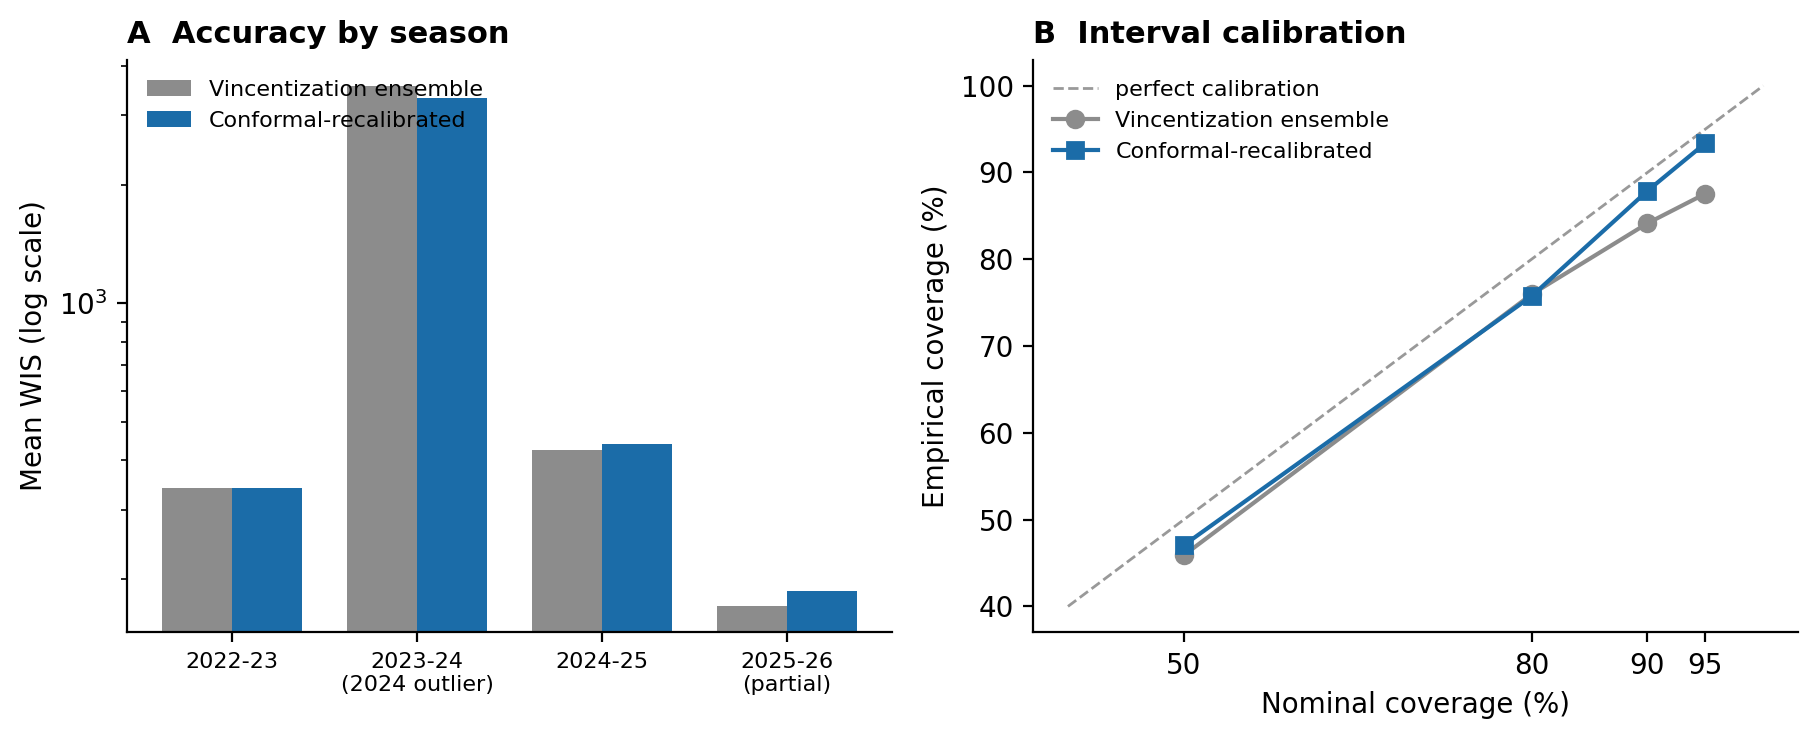
\includegraphics[width=0.92\textwidth]{../results/figures/paper_conformal.png}
\caption{\textbf{Effect of conformal recalibration on the dengue ensemble.} (A) Mean WIS by season,
Vincentization ensemble versus the conformal-recalibrated ensemble (log scale). The gain
concentrates in the 2024 outlier season at a small cost in ordinary seasons. (B) Interval
calibration: empirical versus nominal coverage. Recalibration moves the outer intervals (90, 95)
toward the diagonal.}
\label{fig:conformal}
\end{figure}

\subsection{The winner depends on the evaluation metric}\label{sec:metric}
The overall mean WIS in Table~\ref{tab:leaderboard} is dominated by the largest states and by the
outbreak season, both of which contribute large absolute scores. The challenge's headline metric is
instead a normalized WIS, the sum of WIS divided by the sum of observed cases, which is scale-free
across regions. Under this metric the ordering changes in a revealing way. The conformal ensemble is
best over all folds (normalized WIS 0.555), consistent with the mean-WIS ranking. When the 2024
outlier is excluded to isolate ordinary-season skill, the deep network becomes the best model
(normalized WIS 0.298) while the gradient-boosted model becomes the weakest of the serious models
(0.443), an almost complete reversal of their mean-WIS standing (Fig~\ref{fig:relwis}). The
disagreement is not a paradox. A metric that rewards accuracy on a few very large states favors
different models than one that rewards accuracy on the many small states, and the 2024 season
inflates the mean for whichever model handles it least badly. We therefore report both magnitude-
and unit-weighted skill, and we caution that an epidemic-forecasting leaderboard reporting a single
aggregate can mislead.

\begin{figure}[t]
\centering
\includegraphics[width=0.72\textwidth]{../results/figures/paper_relative_wis.png}
\caption{\textbf{Metric-dependent rankings.} Scale-free relative WIS on the ordinary seasons
compared with magnitude-weighted mean WIS. The single-model ranking reorders: the deep network,
weakest by mean WIS on the outlier, is strongest on ordinary seasons by the scale-free metric.
Figure to be redrawn as an explicit rank-reordering (slope) chart with the current values.}
\label{fig:relwis}
\end{figure}

\subsection{Calibration and its correction}\label{sec:calibration}
Raw gradient-boosted and deep-learning quantile models are over-confident
(Fig~\ref{fig:coverage}). The GRU covers only 32 percent of outcomes in its nominal 50 percent
interval and 75 percent in its nominal 95 percent interval, and it is under-covered in every season
rather than only in the outbreak year, which identifies the problem as systematic overconfidence
rather than a regime-specific failure. Conformalized quantile regression restores the gradient-boosted
model to near-nominal calibration (51/81/89/93) at negligible WIS cost. The same correction applied
to the deep network trades away sharpness on the seasons where it is already accurate, so
calibration and sharpness trade off at the level of a single model. The per-quantile median of the
ensemble provides a structural calibration improvement at no cost, and the conformal recalibration
of Section~\ref{sec:conformal} completes it.

\begin{figure}[t]
\centering
\includegraphics[width=0.6\textwidth]{../results/figures/paper_coverage.png}
\caption{\textbf{Interval calibration by model.} Empirical versus nominal coverage; points on the
diagonal are perfectly calibrated. The deep network is markedly overconfident; conformalized
quantile regression corrects the gradient-boosted model. Figure to be regenerated with the current
model set including the conformal ensemble.}
\label{fig:coverage}
\end{figure}

\subsection{Added complexity did not improve forecasts}\label{sec:negative}
Three interventions that plausibly should have helped did not (Table~\ref{tab:ablation}). First,
adding observed-climate covariates to the gradient-boosted model, following the distributed-lag
non-linear structure of the strongest model in the 2024 sprint \citep{araujo2026,gasparrini2010},
worsened its backtest WIS from 1299 to 1342. A feature-importance analysis showed why: the nine
added covariates (minimum temperature, a derived standardized-precipitation drought index at one,
three, and six month accumulations, multi-month temperature lags, thermal range, and rainy days)
together carried only 5.3 percent of importance and ranked below the existing features. The climate
signal the model actually uses is the seasonal climate forecast and the El Ni\~no--Southern
Oscillation indices, both already present and both forward-looking, rather than observed local
weather, which is stale at the long horizons that dominate a full-season forecast. Second, a
hierarchical, empirical-Bayes pooling of each state's seasonal climatology toward its macroregion
worsened the ensemble from 1216 to 1241, because Brazilian states are too heterogeneous within a
macroregion: shrinking a small state toward a region dominated by a larger, differently behaving
state introduces bias. Third, a hyperparameter search that improved an internal time-block holdout
by 5 percent worsened the true backtest, because an internal holdout does not represent forecasting
a full future season from mid-year. Conservative, a priori defaults generalized better. Together
these results locate the predictable signal in this problem and caution against complexity that is
not validated on the true forecasting task.

\begin{table}[t]
\centering\small
\caption{\textbf{Interventions that did not help (negative results).} Each was evaluated on the same
backtest as the main comparison.}
\label{tab:ablation}
\begin{tabular}{@{}lll@{}}
\toprule
\textbf{Intervention} & \textbf{Effect} & \textbf{Reason} \\
\midrule
Observed-climate covariates (LightGBM) & WIS 1299 $\rightarrow$ 1342 & 5.3\% importance; signal is climate \\
 & & forecast + ENSO, not observed weather \\
Hierarchical macroregion pooling & WIS 1216 $\rightarrow$ 1241 & small-state bias; too correlated \\
 (added to ensemble) & & with climatological member \\
Hyperparameter tuning & internal holdout $+5\%$, & internal holdout misrepresents \\
 & backtest worse & full-season forecasting \\
\bottomrule
\end{tabular}
\end{table}

\subsection{The best model is disease-specific}\label{sec:chik}
For chikungunya, evaluated on the same harness and states, the gradient-boosted model alone is the
best forecaster (WIS 82.3), ahead of the ensemble (91.6) and every other model
(Table~\ref{tab:chik}). It dominates every season, so combining it with weaker models only dilutes
it. The contrast with dengue, where the ensemble wins, shows that the choice of forecasting model
should be made per target rather than assumed to transfer across diseases, even within the same
surveillance system and pipeline.

\begin{table}[t]
\centering\small
\caption{\textbf{Chikungunya backtest.} State-level, same harness and seasons as dengue. Gradient
boosting alone is best.}
\label{tab:chik}
\begin{tabular}{@{}lrcc@{}}
\toprule
\textbf{Model} & \textbf{WIS} & \textbf{Cov.\ 50 (\%)} & \textbf{Cov.\ 90 (\%)} \\
\midrule
LightGBM                  & \textbf{82.3} & 45 & 87 \\
Ensemble (Vincentization) & 91.6 & 53 & 87 \\
Climatological            & 94.4 & 55 & 84 \\
Seasonal-naive            & 97.8 & 49 & 89 \\
Mechanistic               & 101.0 & 51 & 85 \\
Naive                     & 123.1 & 40 & 79 \\
\bottomrule
\end{tabular}
\end{table}

\section{Discussion}

\subsection{Robustness under regime shift}
The most consequential finding is that model rankings are season-dependent and can invert in an
outbreak year. A model chosen for its average score can be the least reliable in the season for which
forecasts matter most, as the deep network is here. Two responses follow. One is to combine models,
so that no single failure mode determines the forecast; the ensemble is never worst in any season
and is best overall once recalibrated. The other is to prefer models whose uncertainty widens under
distribution shift, as the mechanistic model's bootstrap-of-historical-seasons intervals do. These
observations align with evidence from collaborative forecast hubs, where combined forecasts are
consistently competitive with or better than their members \citep{cramer2022,reich2019,sherratt2023}.

\subsection{Metric choice is a reporting-standards issue}
The identity of the best model changes with the aggregation of skill across a highly skewed set of
states. This is not specific to our models or to Brazil. Any national forecasting evaluation with
strong heterogeneity in population and incidence faces the same tension between magnitude-weighted
and unit-weighted skill. Reporting a single aggregate obscures it. We recommend reporting both, as
the interval-score and forecast-hub literature increasingly does \citep{bracher2021}, and we treat
the normalized WIS the challenge adopts as the headline while retaining magnitude-weighted mean WIS
and per-unit relative WIS alongside it.

\subsection{Simple methods and the limits of complexity}
Deep learning did not dominate, and simple methods, a climatological quantile model and a bootstrap
of historical seasons, were hard to beat. This is consistent with forecasting-competition evidence
that in small-sample, few-series regimes, parsimonious methods and combinations are strong
\citep{makridakis2020}. Our negative results sharpen the point. The covariate that helped the
strongest 2024-sprint model, climate acting through a distributed-lag non-linear response
\citep{lowe2021,gasparrini2010}, did not help our gradient-boosted forecaster, because that
structure requires the regularized, partially pooled Bayesian formulation in which it was developed,
whereas an unregularized tree over the same inputs overfits low-signal dimensions. The forecast-relevant
climate information in our pipeline is the seasonal forecast and large-scale oscillation indices, not
observed local weather. This clarifies where future modeling effort should go: toward a Bayesian
spatiotemporal member that can use climate through an exposure-lag-response surface, rather than
toward more covariates in a boosted model.

\subsection{Conformal recalibration as transferable insurance}
The conformal recalibration is simple, scale-free, and cheap, and it improves both accuracy and
calibration. It connects to conformalized quantile regression \citep{romano2019} and to adaptive
conformal methods for distribution shift \citep{gibbs2021}, and it matches the online-recalibration
result reported for probabilistic dengue forecasting elsewhere. Because it widens mainly the outer
tails, it protects against the failure mode that dominates the outbreak season without materially
degrading ordinary-season sharpness. For an operational forecaster who cannot know in advance whether
the coming season will be ordinary or extreme, this asymmetric protection is the right default.

\subsection{Limitations}
The fourth backtest season is only partially resolved in the available data and is reported
separately; its numbers will firm up as the 2025--26 season completes. Municipality-to-state
aggregation discards sub-state epidemic asynchrony that a municipal model could exploit. The study
covers two diseases in one country and is retrospective; a true prospective evaluation awaits the
challenge's forecast phase. The comparison is single-team, so it does not capture the full diversity
of approaches a multi-team sprint would, and the conformal factors are calibrated on one season under
the challenge's tuning-fold discipline rather than by a fully online procedure.

\subsection{Future work}
The immediate next step is the challenge forecast phase, which will provide a genuine prospective
score for the recalibrated ensemble on the 2026--27 season. Beyond it, three directions follow from
our results: a Bayesian spatiotemporal member with a distributed-lag non-linear climate response,
which our negative result suggests is the right home for climate covariates; hierarchical
reconciliation across state, city, and national forecasts for coherence; and municipal-level feature
engineering for the optional city tracks.

\section{Materials and methods}\label{sec:methods}

\subsection{Data and targets}
Weekly dengue and chikungunya case counts per municipality (2010--2026) are drawn from the Infodengue
system, which harmonizes notifiable-disease surveillance \citep{codeco2018}, and aggregated to the 26
mandatory states, excluding Espírito Santo per the challenge. Covariates comprise weekly climate
reanalysis (temperature, precipitation, humidity, pressure, thermal range, rainy days), a seasonal
climate forecast, ocean-oscillation indices (El Ni\~no--Southern Oscillation, Indian Ocean Dipole,
Pacific Decadal Oscillation), yearly municipal population, and static climate-zone and biome
covariates. The forecasting target is the weekly state case count over each season, submitted as the
nine quantiles 0.025, 0.05, 0.10, 0.25, 0.50, 0.75, 0.90, 0.95, and 0.975.

\subsection{Backtest design and leakage control}
The four official seasons are derived at runtime from the challenge's train and target flags. A
confirmed 15-week gap separates each training cutoff from the start of its evaluation window,
simulating reporting delay. Two leakage disciplines are enforced centrally in the harness rather than
in individual models. All covariate access is filtered to dates at or before the training cutoff, and
lag and rolling features are computed from the continuous cutoff-filtered history rather than from the
gapped target window. Both are checked by automated regression tests, so a leak would fail the test
suite rather than silently inflate scores.

\subsection{Scoring}\label{sec:methods-scoring}
Forecasts are scored by the weighted interval score,
\[
\mathrm{WIS}(F,y)=\frac{1}{K+\tfrac12}\Big[\tfrac12\,|y-m|+\sum_{k=1}^{K}\frac{\alpha_k}{2}\,
\mathrm{IS}_{\alpha_k}(\ell_k,u_k,y)\Big],
\]
over the four required central intervals, where $m$ is the predictive median, $\mathrm{IS}_{\alpha}$
is the interval score at level $1-\alpha$, and the weights reproduce the mean pinball loss over the
nine required quantiles, the exact discrete approximation to the continuous ranked probability score
\citep{gneiting2007,bracher2021}. Our implementation is verified against the challenge platform's own
scorer. We also report empirical interval coverage, a decomposition of WIS into dispersion and
directional (over- and under-prediction) penalties, a scale-free per-unit relative WIS, and the
normalized WIS (sum of WIS divided by sum of observed cases) that the challenge adopts as its headline
metric.

\subsection{Models}
\textbf{Baselines.} A naive model (last observed value with empirical horizon-difference quantiles), a
seasonal-naive model (same-epidemiological-week history), and a climatological quantile model (direct
order-statistic quantiles per state and epidemiological week over a five-week window).

\noindent\textbf{Gradient boosting.} A LightGBM quantile-regression model \citep{ke2017} fit on a
synthetic-origin panel that expands each fold into many weekly origins crossed with forecast horizons,
with origin-anchored lag, rolling, seasonal, climate, ocean, seasonal-forecast, and static features.
Predictive intervals are calibrated by conformalized quantile regression \citep{romano2019}.

\noindent\textbf{Deep learning.} A global gated recurrent unit (GRU) network \citep{cho2014} with
per-state embeddings and a negative-binomial output head, trained as a deep ensemble of
independently seeded runs \citep{lakshminarayanan2017}; quantiles are analytic from the negative-binomial
predictive distribution and pooled across ensemble members by quantile averaging.

\noindent\textbf{Semi-mechanistic.} A model that bootstraps historical season trajectories under a
negative-binomial observation model, a local reimplementation of Richards-curve epidemic-scanner fits
\citep{richards1959}, producing wide, well-calibrated intervals under distribution shift.

\noindent\textbf{Ensembles.} Models are combined by per-quantile median (Vincentization) and by
inverse-WIS weights tuned only on the designated tuning season, so weights are never fit on the
seasons on which the ensemble is reported.

\subsection{Conformal recalibration}\label{sec:methods-conformal}
For each central interval level $L$ with bounds $[\ell_L,u_L]$ and median $m$, we compute a
multiplicative widening factor $s_L$ that makes the interval reach its nominal coverage on the tuning
season. For each calibration unit, the multiple needed to just cover the observation is
$r=(y-m)/(u_L-m)$ when $y>m$ and $r=(m-y)/(m-\ell_L)$ when $y<m$; $s_L$ is the $L/100$ empirical
quantile of $r$, a scale-free, multiplicative analogue of conformalized quantile regression that is
robust to the large cross-state differences in scale. The interval is then widened about the median
by $s_L$, and monotonicity across quantiles is restored by a rearrangement step. Factors are estimated
on the tuning season and applied to all seasons; recalibrating the ensemble output outperforms
recalibrating any single member. For the forecast phase, the factors are to be estimated on all four
validation seasons and applied to the prospective forecast.

\subsection{Reproducibility}
All code, the backtesting harness, per-state scored predictions, and validated submission files for
four official tracks (dengue and chikungunya, state and city level) are released. The pipeline is
deterministic under a fixed seed, and an automated test suite covers leakage safety, scoring
correctness, model persistence, and every model family. A provenance manifest records the exact data
and code state behind each reported number. The Supporting Information provides the full feature list
and frozen hyperparameters, the deep-learning architecture, the mechanistic derivation, per-state and
per-fold tables, the ensemble-member and weight robustness analysis, and an item-by-item EPIFORGE 2020
reporting checklist \citep{pollett2021}.

\section*{Data and code availability}
All code, data-processing pipeline, backtests, figures, and validated submissions are openly
available at the project repository (URL to be inserted on submission).

\bibliographystyle{unsrtnat}
\begin{thebibliography}{99}
\small
\bibitem{araujo2026} Araujo EC, Carvalho LM, Coelho FC, et al. Leveraging probabilistic forecasts for dengue preparedness and control: the 2024 Dengue Forecasting Sprint in Brazil. \emph{Proc Natl Acad Sci USA} (2026).
\bibitem{bracher2021} Bracher J, Ray EL, Gneiting T, Reich NG. Evaluating epidemic forecasts in an interval format. \emph{PLoS Comput Biol} 17(2):e1008618 (2021).
\bibitem{gneiting2007} Gneiting T, Raftery AE. Strictly proper scoring rules, prediction, and estimation. \emph{J Am Stat Assoc} 102(477):359--378 (2007).
\bibitem{romano2019} Romano Y, Patterson E, Cand\`es EJ. Conformalized quantile regression. \emph{Adv Neural Inf Process Syst} 32 (2019).
\bibitem{gibbs2021} Gibbs I, Cand\`es EJ. Adaptive conformal inference under distribution shift. \emph{Adv Neural Inf Process Syst} 34 (2021).
\bibitem{ke2017} Ke G, Meng Q, Finley T, et al. LightGBM: a highly efficient gradient boosting decision tree. \emph{Adv Neural Inf Process Syst} 30 (2017).
\bibitem{cho2014} Cho K, van Merri\"enboer B, Gulcehre C, et al. Learning phrase representations using RNN encoder-decoder for statistical machine translation. \emph{Proc EMNLP} (2014).
\bibitem{lakshminarayanan2017} Lakshminarayanan B, Pritzel A, Blundell C. Simple and scalable predictive uncertainty estimation using deep ensembles. \emph{Adv Neural Inf Process Syst} 30 (2017).
\bibitem{gasparrini2010} Gasparrini A, Armstrong B, Kenward MG. Distributed lag non-linear models. \emph{Stat Med} 29(21):2224--2234 (2010).
\bibitem{lowe2021} Lowe R, Lee SA, O'Reilly KM, et al. Combined effects of hydrometeorological hazards and urbanisation on dengue risk in Brazil. \emph{Lancet Planet Health} 5(4):e209--e219 (2021).
\bibitem{cramer2022} Cramer EY, Ray EL, Lopez VK, et al. Evaluation of individual and ensemble probabilistic forecasts of COVID-19 mortality in the United States. \emph{Proc Natl Acad Sci USA} 119(15):e2113561119 (2022).
\bibitem{reich2019} Reich NG, Brooks LC, Fox SJ, et al. A collaborative multiyear, multimodel assessment of seasonal influenza forecasting in the United States. \emph{Proc Natl Acad Sci USA} 116(8):3146--3154 (2019).
\bibitem{sherratt2023} Sherratt K, Gruson H, Grah R, et al. Predictive performance of multi-model ensemble forecasts of COVID-19 across European nations. \emph{eLife} 12:e81916 (2023).
\bibitem{pollett2021} Pollett S, Johansson MA, Reich NG, et al. Recommended reporting items for epidemic forecasting and prediction research: the EPIFORGE 2020 guidelines. \emph{PLoS Med} 18(10):e1003793 (2021).
\bibitem{johansson2019} Johansson MA, Apfeldorf KM, Dobson S, et al. An open challenge to advance probabilistic forecasting for dengue epidemics. \emph{Proc Natl Acad Sci USA} 116(48):24268--24274 (2019).
\bibitem{codeco2018} Codeço CT, Coelho F, Cruz O, et al. Infodengue: a nowcasting system for the surveillance of arboviruses in Brazil. \emph{Rev Saude Publica} (2018).
\bibitem{lowe2021b} Lowe R, et al. Nonlinear and delayed impacts of climate on dengue risk in Barbados. \emph{PLoS Med} 15(7):e1002613 (2018).
\bibitem{makridakis2020} Makridakis S, Spiliotis E, Assimakopoulos V. The M4 competition: 100,000 time series and 61 forecasting methods. \emph{Int J Forecast} 36(1):54--74 (2020).
\bibitem{colon2021} Col\'on-Gonz\'alez FJ, Sewe MO, Tompkins AM, et al. Projecting the risk of mosquito-borne diseases in a warmer and more populated world. \emph{Lancet Planet Health} 5(7):e404--e414 (2021).
\bibitem{richards1959} Richards FJ. A flexible growth function for empirical use. \emph{J Exp Bot} 10(2):290--301 (1959).
\end{thebibliography}

\end{document}
